\chapter{Background knowledge}
\label{sec:background}

Before attempting to answer our research questions, it is necessary to explain the relevant parts of Ask-Elle's architecture. This chapter presents the concepts of \emph{programming strategy} and \emph{program unification}.

\section{Programming strategies}

As mentioned in Chapter \ref{sec:intro}, an exercise in Ask-Elle is a request to implement a function that matches one of the model solutions. Under the hood, Ask-Elle  generates a \emph{programming strategy} that specifies how an exercise can be solved, as a series of steps that go from an empty program to one of the model solutions.

Alternatively, we can think of a strategy as a finite-state machine. The initial state is the empty program, the transitions are the refinement steps and the accepting states are the model solutions.

Consider, for example, the model solution to the problem presented in Section \ref{sec:intro-askelle-example-session} (defined as \mintinline{haskell}{double = map (* 2)}). Figure \ref{fig:bg-fsm-prog-strategies} shows the generated strategy.

\begin{figure}
\centering
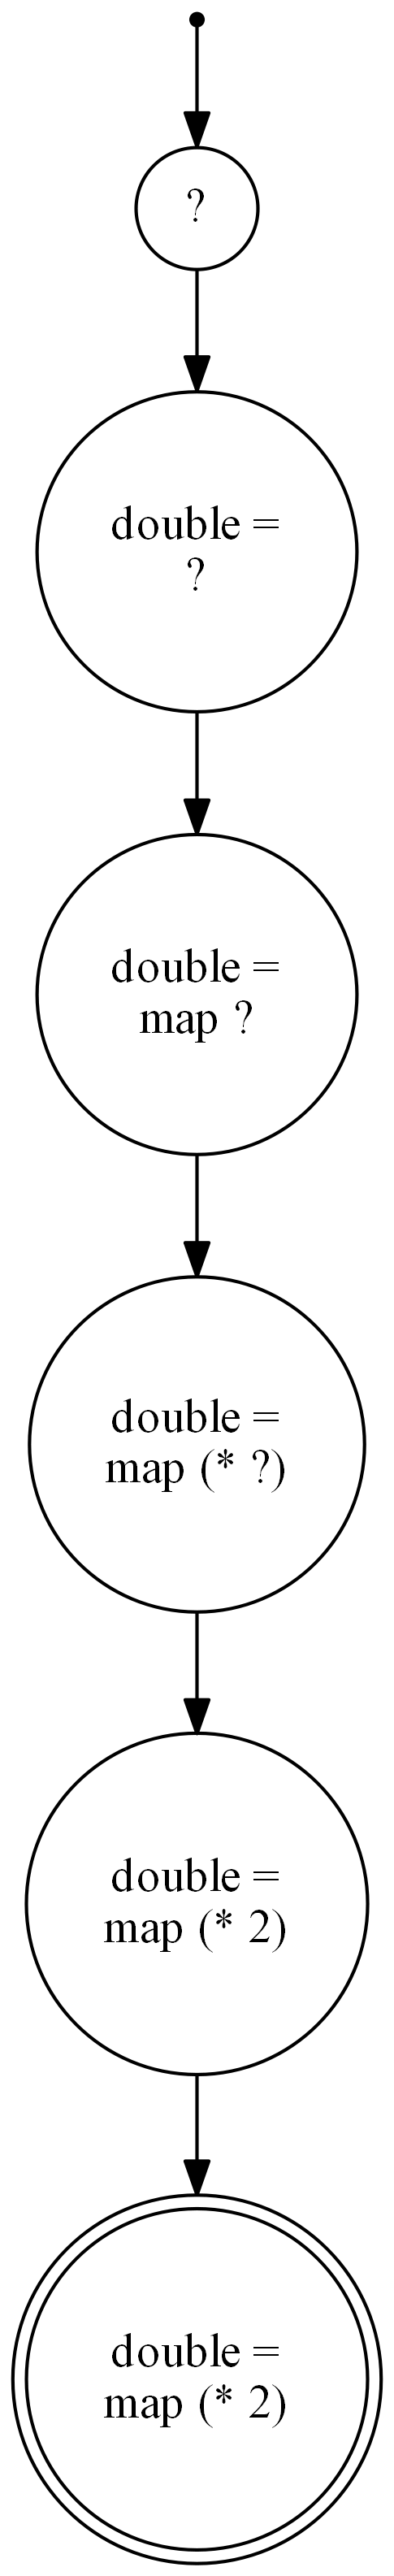
\includegraphics[height=20cm]{graphs/bg-fsm-prog-strategies}
\caption{Example of an Ask-Elle strategy}
\label{fig:bg-fsm-prog-strategies}
\end{figure}

According to the finite-state machine perspective on strategies, the algorithm used by Ask-Elle to provide hints works in two steps:

\begin{enumerate}
    \item Translate the student's program to a state in the machine;
    \item Retrieve a list of all transitions available from that state and present them in a user-friendly fashion.
\end{enumerate}

From these two steps, the second is a common operation on finite-state machines. The first one, however, is much more involved, as it requires unifying programs.

\section{Program unification}

The process of comparing two programs for semantic equivalence up to holes is called program unification. This is what Ask-Elle does when comparing a student program to a model solution.

Since the problem of program unification is undecidable in the case of a complex language such as Haskell (see Section \ref{sec:related-work-unification}), Ask-Elle's unification procedure has the following possible outcomes:

\begin{enumerate}
    \item The programs are semantically equivalent;
    \item One program is an incomplete version of the other;
    \item Equivalence cannot be concluded.
\end{enumerate}

At the core of Ask-Elle's unification mechanism is the idea of normalization. Before comparing the programs, they go through a series of semantics-preserving transformations that result in a normal form. This way, comparing the programs becomes as simple as syntactically unifying the resulting normal forms.

Consider, for instance, the \texttt{double} function we have been referring to throughout this proposal. Figure \ref{fig:bg-unification-normalization} shows a model solution, a possible student answer and the normalized version of both programs. This is an example of how a small syntactical difference, an unnecessary anonymous function, is ignored thanks to semantics-preserving transformations.

\begin{figure}[H]
\begin{minted}{haskell}
-- Model solution
double = map (* 2)

-- Student answer
double = map (\x -> 2 * x)

-- Normalized version (similar for both)
double = map ((*) 2)
\end{minted}
\caption{Example of unification by normalization}
\label{fig:bg-unification-normalization}
\end{figure}
